\documentclass[
  xcolor=svgnames,
  bookmarks=true,
  bookmarksopen=true,
  pdfborder={0 0 0},
  pdfhighlight={/N},
  linkbordercolor={rgb}{0.5,0.5,0.5},
  implicit=false,
  colorlinks=true,
  allcolors=deepblue
]{beamer}

\usepackage[utf8]{inputenc}
\usepackage{booktabs, comment}
\usepackage{pgfpages}
\usepackage{ragged2e}
\usepackage{csquotes}
\usepackage{graphicx}
\usepackage{amsmath}
\usepackage{tikz}
\usepackage{natbib}
\renewcommand{\bibfont}{\small}
\setlength{\bibsep}{2pt}


\definecolor{royalblue}{RGB}{70, 130, 180}
\usecolortheme[named=royalblue]{structure}

\setbeamercolor{frametitle}{fg=white, bg=royalblue}
\setbeamertemplate{frametitle}[default][left]
\setbeamercolor{title in head/foot}{bg=lightgray, fg=black}
\setbeamercolor{section in toc}{fg=royalblue}
\setbeamercolor{section in head/foot}{bg=royalblue, fg=white}
\setbeamercolor{page number in head/foot}{bg=royalblue, fg=white}
% TITLE, AUTHORS, INSTITUTE, DATE

\title[When Nature Strikes]{\textbf{When Nature Strikes: Firm Responses to Environmental Disasters in India}}
\author[Benoît Chaulvet]{Benoît Chaulvet}
\institute[Université Paris 1]{Paris 1 Pantheon-Sorbonne University}
\date{June 12th, 2025}

\makeatletter
\setbeamertemplate{footline}{
  \leavevmode%
  \hbox{% 
  \begin{beamercolorbox}[wd=.5\paperwidth,ht=2.25ex,dp=1ex,center]{author in head/foot}%
    \usebeamerfont{author in head/foot}\insertshortauthor
  \end{beamercolorbox}%
  \begin{beamercolorbox}[wd=.4\paperwidth,ht=2.25ex,dp=1ex,center]{title in head/foot}%
    \usebeamerfont{title in head/foot}\insertshorttitle
  \end{beamercolorbox}%
  \begin{beamercolorbox}[wd=.1\paperwidth,ht=2.25ex,dp=1ex,right]{page number in head/foot}%
    \usebeamerfont{page number in head/foot}\insertframenumber{} / \inserttotalframenumber\hspace*{2ex}
  \end{beamercolorbox}}%
  \vskip0pt%
}
\makeatother
\beamertemplatenavigationsymbolsempty

\titlegraphic{
\includegraphics[height=1.5cm]{Logo Paris 1.png}}

\newcommand{\customtitlepage}{
\begin{frame}[plain]
  \begin{tikzpicture}[remember picture,overlay]
    \fill[royalblue] (current page.south west) rectangle (current page.north east);
  \end{tikzpicture}

  \vspace*{1.5cm}
  \color{white}
  \centering
  {\Huge \textbf{\inserttitle}}\\[1cm]
  {\Large \insertauthor}\\[0.3cm]
  {\large \insertinstitute}\\[0.5cm]
  {\normalsize \insertdate}
  \vfill
  
\includegraphics[height=1.5cm]{Logo Paris 1.png}
\end{frame}
}

\begin{document}

\begin{frame}
    \titlepage
\end{frame}

\begin{frame}{Introduction}
\large
{\setbeamertemplate{itemize items}[circle]
\textbf{Motivations}
\begin{itemize}
    \item Rise of economic damages linked to environmental disasters
    \item Why India is an interesting case?
    \item policy driven: \textit{"Our house burns and we look elsewhere"} (Chirac, 2002)
\end{itemize}
}
\end{frame}


\begin{frame}{Theoretical channels}
\large
{\setbeamertemplate{itemize items}[circle]
\textbf{Theoretical Channels}
\begin{itemize}
    \item Capital \& Labor disruptions $\Rightarrow$ Productivity decrease $\Rightarrow$ Performance drops
    \item Demand shocks depending on the industry
    \item Imported inputs can mitigate damages (less affected than domestic inputs)
\end{itemize}
}
\end{frame}


\begin{frame}{Contributions to the Literature}
\begin{itemize}
    \item \textbf{Unclear relationship between disasters and growth}
    {\setbeamertemplate{itemize subitem}[circle]
    \begin{itemize}
        \item Builds on the literature documenting the effect of disasters on the economy ({\footnotesize\cite{RothTran2025, Okubo2021, Collati2024, friedt2022}})
        \item \textbf{Contributions:} Micro-level data + Developing country
    \end{itemize}
    }

\vspace{0.3cm}
    \item \textbf{Environmental shock on firm performance}
    {\setbeamertemplate{itemize subitem}[circle]
    \begin{itemize}
        \item Identifies the drivers of performance decrease for affected firms ({\footnotesize\cite{Bas2025, Nedoncelle2024, Barrot2016}})
        \item \textbf{Contributions:} Sector heterogeneity + Value added
    \end{itemize}
    }

\vspace{0.3cm}
    \item \textbf{Adaptation mechanisms to disasters}
    {\setbeamertemplate{itemize subitem}[circle]
    \begin{itemize}
        \item Highlights a less explored adaptation mechanism ({\footnotesize\cite{Henriet2012, Nedoncelle2024, Hsu2018}})
        \item \textbf{Contributions:} Role of foreign inputs and international networks
    \end{itemize}
    }
\end{itemize}
\end{frame}


\begin{frame}{At a First Glance}
\centering
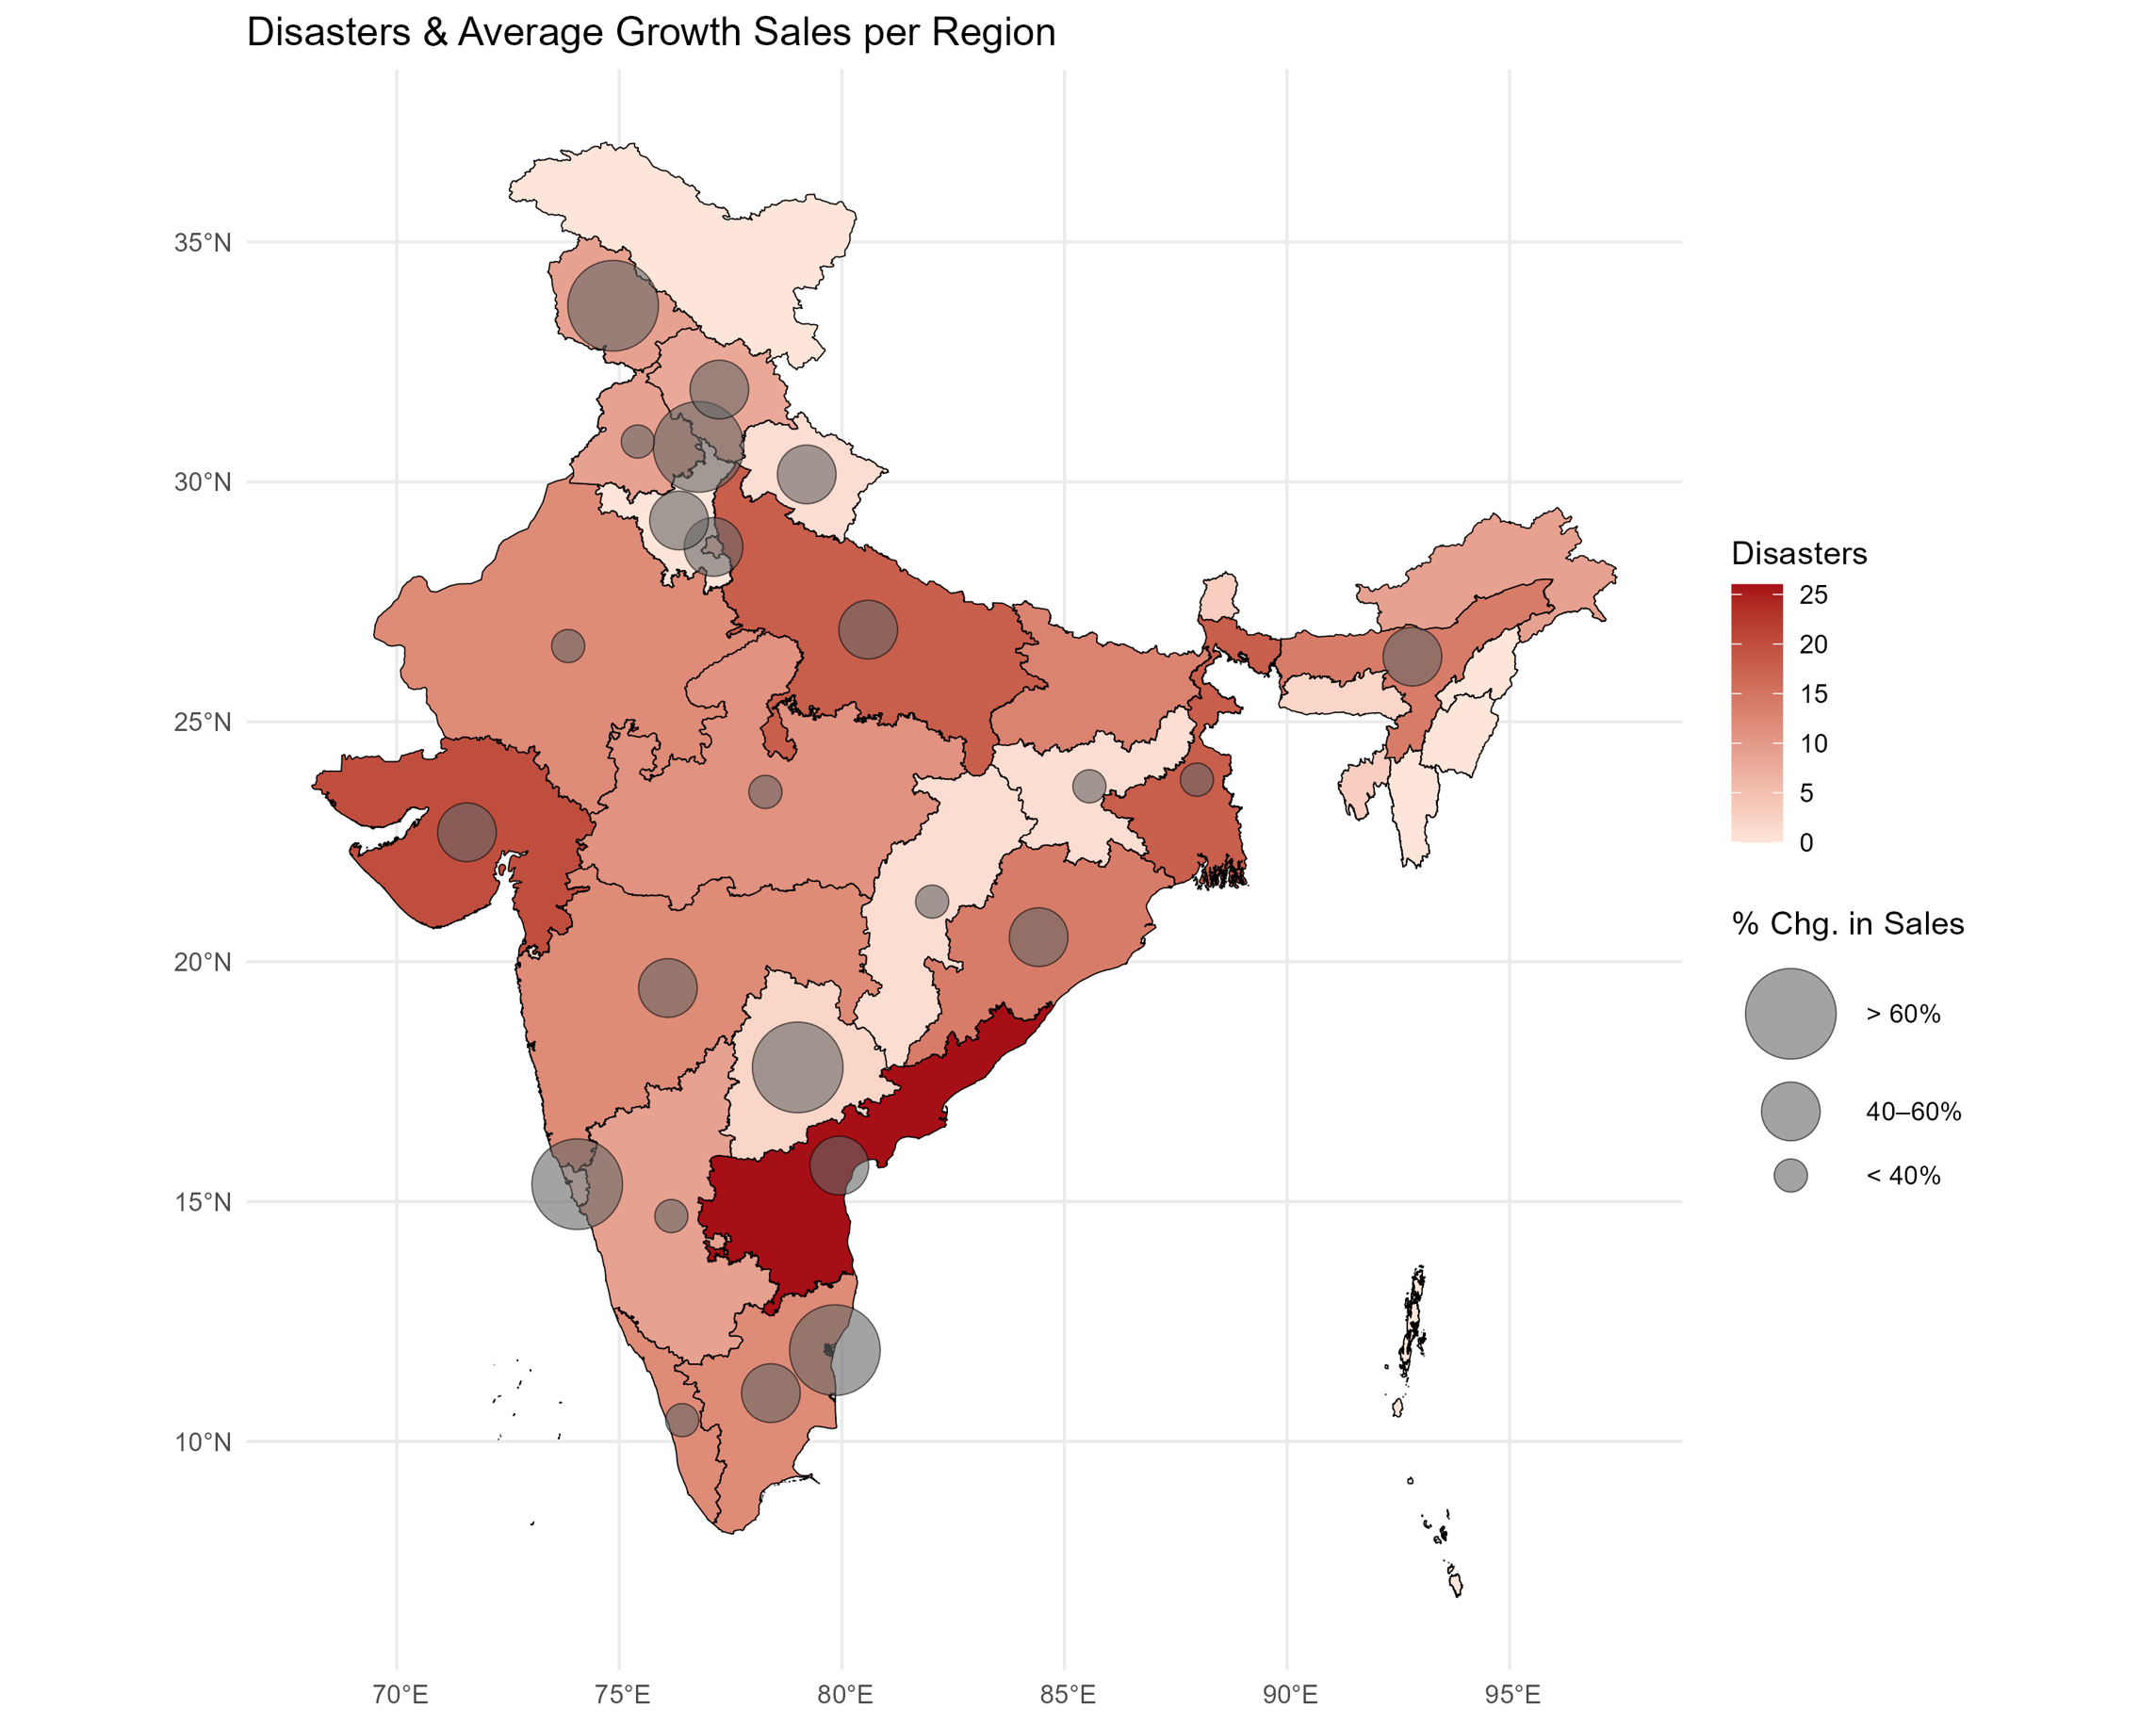
\includegraphics[height=7 cm]{Map disasters.png}
\begin{itemize}
    \item Shows disaster frequency and average sales growth (1990--2006)
\end{itemize}
\end{frame}

\begin{frame}{Data and Sources}
\begin{itemize}
    \item \textbf{Firm data:} Prowess (CMIE)
     {\setbeamertemplate{itemize subitem}[circle]
    \begin{itemize}
        \item Study period 1990--2006
        \item Financial performance of Indian Firms
        \item \textbf{Geolocated} with pinpoints
    \end{itemize}
    }
\vspace{0.3cm}
\item \textbf{Disaster data:} EM-DAT (CRED)
 {\setbeamertemplate{itemize subitem}[circle]
    \begin{itemize}
        \item Start \& End date
        \item Type of disaster, Number of people affected + Economic damages
        \item \textbf{District / Province location}
    \end{itemize}
    }
\vspace{0.3cm}
\item \textbf{Merging Key}: Indian Postal Code Directory

\end{itemize}
\end{frame}

\begin{frame}{Descriptive Statistics}
\vspace{-1cm}
\begin{minipage}{1.1\textwidth}
    \centering
    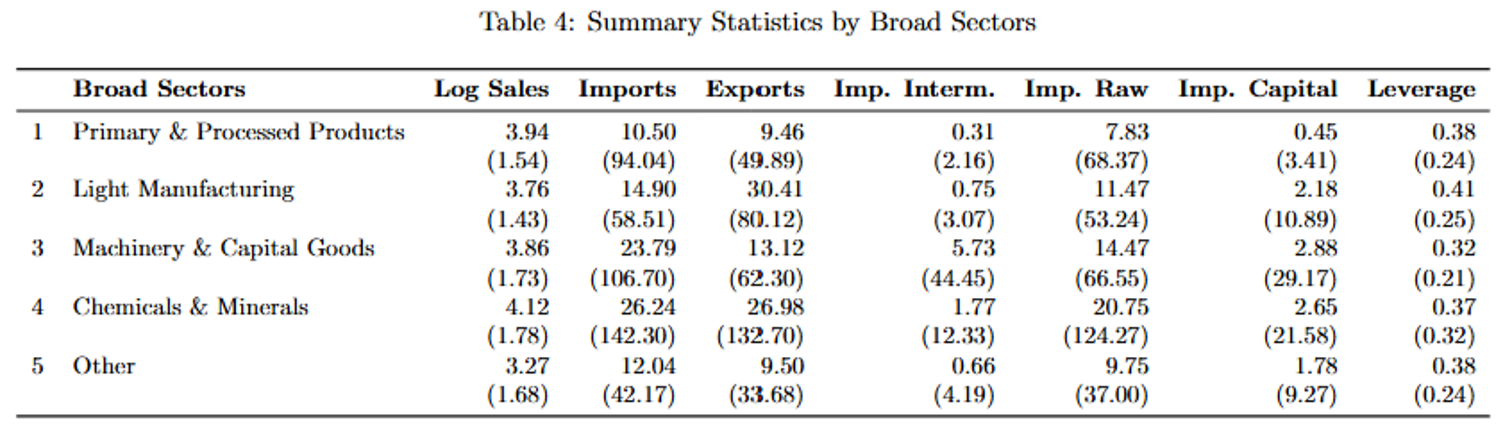
\includegraphics[width=\linewidth]{Summary Stat sectors.png}
\end{minipage}
\vspace{0.5cm}
\begin{itemize}
    \item \textbf{3,245} firms, \textbf{26,133 observations}
    \item 13 Industries merged into \textbf{Broader Categories using the ISIC Rev 4 classifications (United Nations)}
    \item Increase of the key variables over time (cf Appendices)
    \item Import values are greater for firms in downstream industries
\end{itemize}
\end{frame}

\begin{frame}{Identification Strategy}

\textbf{Event Study framework with PSM matching}
\centering
\begin{align}
\text{lsales}_{it} =\ & \sum_{t = -3,\, t \ne -1}^{5} \beta_t \cdot \text{event}_{kit} + \omega \cdot \text{X}_{it}'\nonumber \\
&
+ \gamma_1 \cdot \text{droughts\_cumulative}_{pt}
+ \gamma_2 \cdot \text{floods\_cumulative}_{pt} \nonumber \\
& + \gamma_3 \cdot \text{cyclones\_cumulative}_{pt}
+ \alpha_i + \delta_{st} + \psi_{gt} + \varepsilon_{it}
\end{align}

\scriptsize
\begin{itemize}
    \item $Y_{it}$:  Outcome variables  $Firm_{i}$ performance (Sales, wages, productivity)
    \item $Event_{kit}$: 8 dummies representing the time periods before and after the $disaster_ {k}$ (event t-1 is dropped)
    \item $X_{it}$: Firm characteristics (Productivity, Energy expenses, leverage)
    \item Cumulative $disasters_{pt}$: Time varying variable capturing anticipation behaviors
    \item $\alpha_{st}$: $sector_{s}$-year fixed effects
    \item $\delta_{i}$: Firm fixed effect
    \item $\psi_{gt}$: $group_{g}$-$year_{t}$ Fixed effects

\end{itemize}

\end{frame}

\begin{frame}{Event Study Results}
\centering
\begin{minipage}{0.49\textwidth}
    \centering
    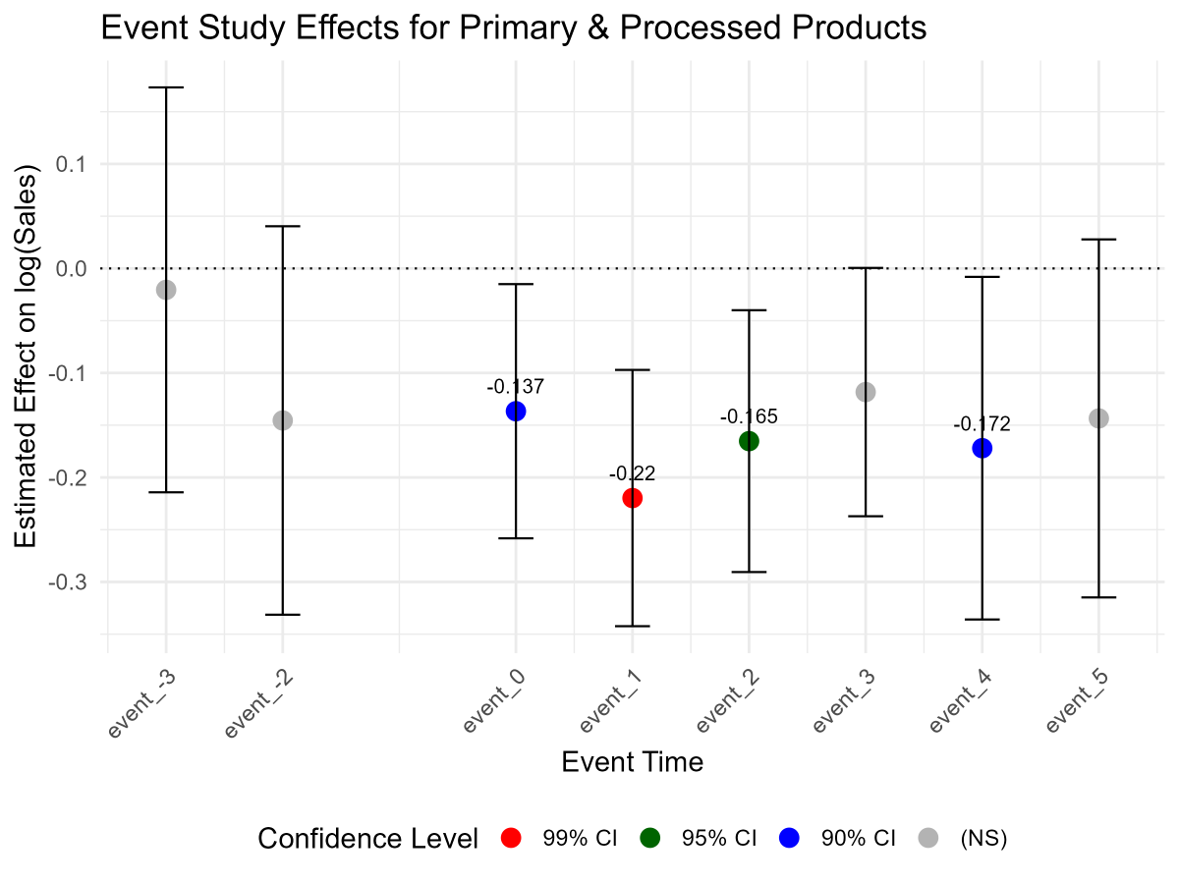
\includegraphics[width=\linewidth]{Results Prim.png}
\end{minipage}
\hfill
\begin{minipage}{0.49\textwidth}
    \centering
    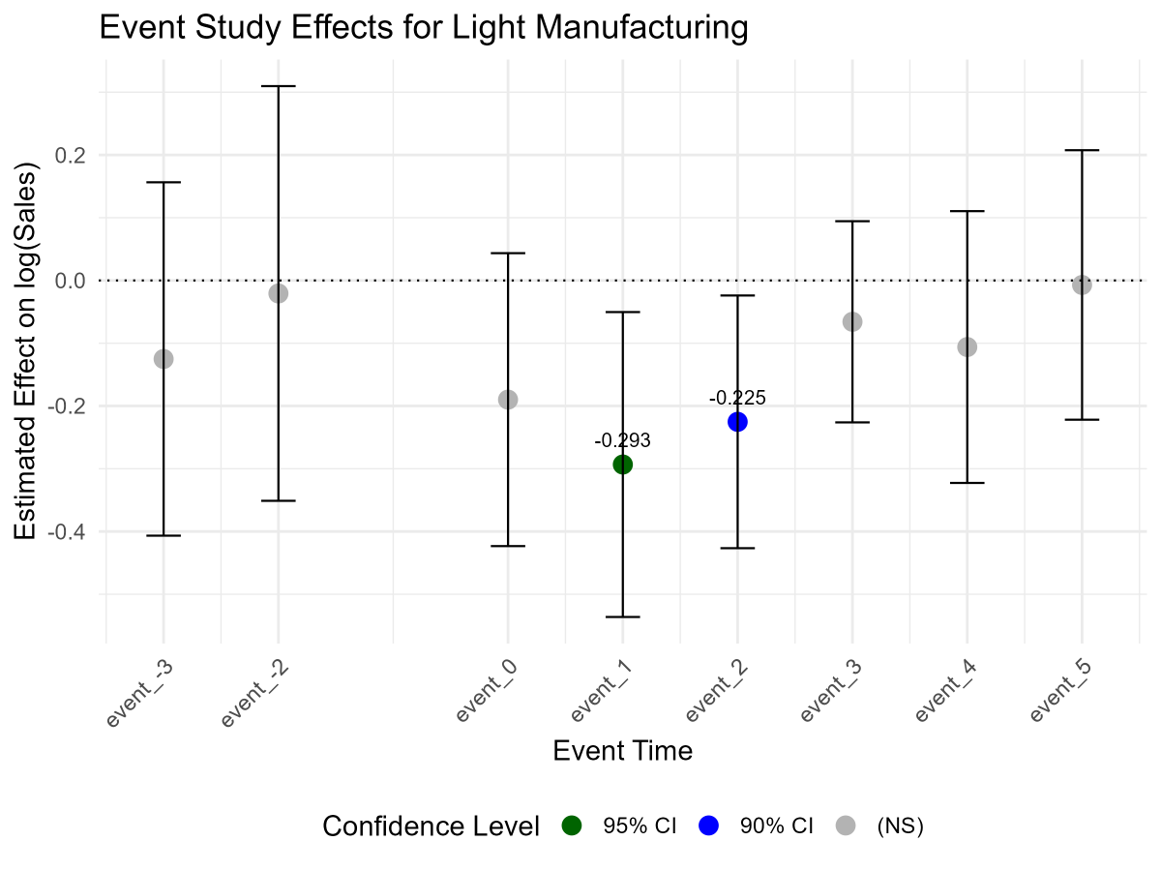
\includegraphics[width=\linewidth]{Results Manuf.png}
\end{minipage}
\vspace{0.5cm}
\begin{itemize}
    \item Significant drop in sales in Primary \& Processed Products and Light Manufacturing

\end{itemize}
\end{frame}

\begin{frame}{Event Study Results -- Magnitude}

\centering
    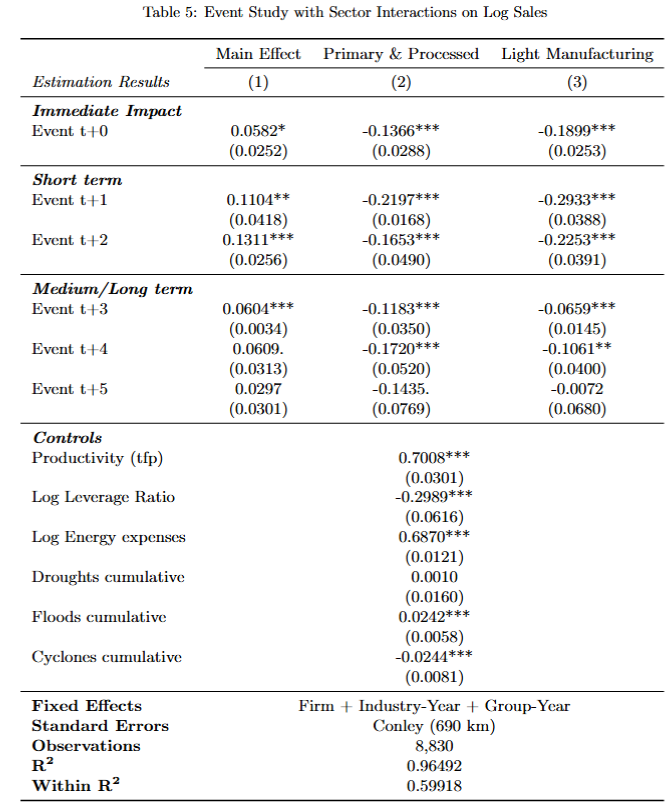
\includegraphics[height = 7 cm]{Table Results Prim and Manuf.png}
\begin{itemize}
\scriptsize
    \item Compared to Baseline industry (Chemicals \& Minerals) \textbf{10\% to 29\%}
    \item Compared to non-treated siblings \textbf{8\% to 18\%}
\end{itemize}
\end{frame}


\begin{frame}{Mechanisms}
\centering
\begin{minipage}{0.49\textwidth}
    \centering
    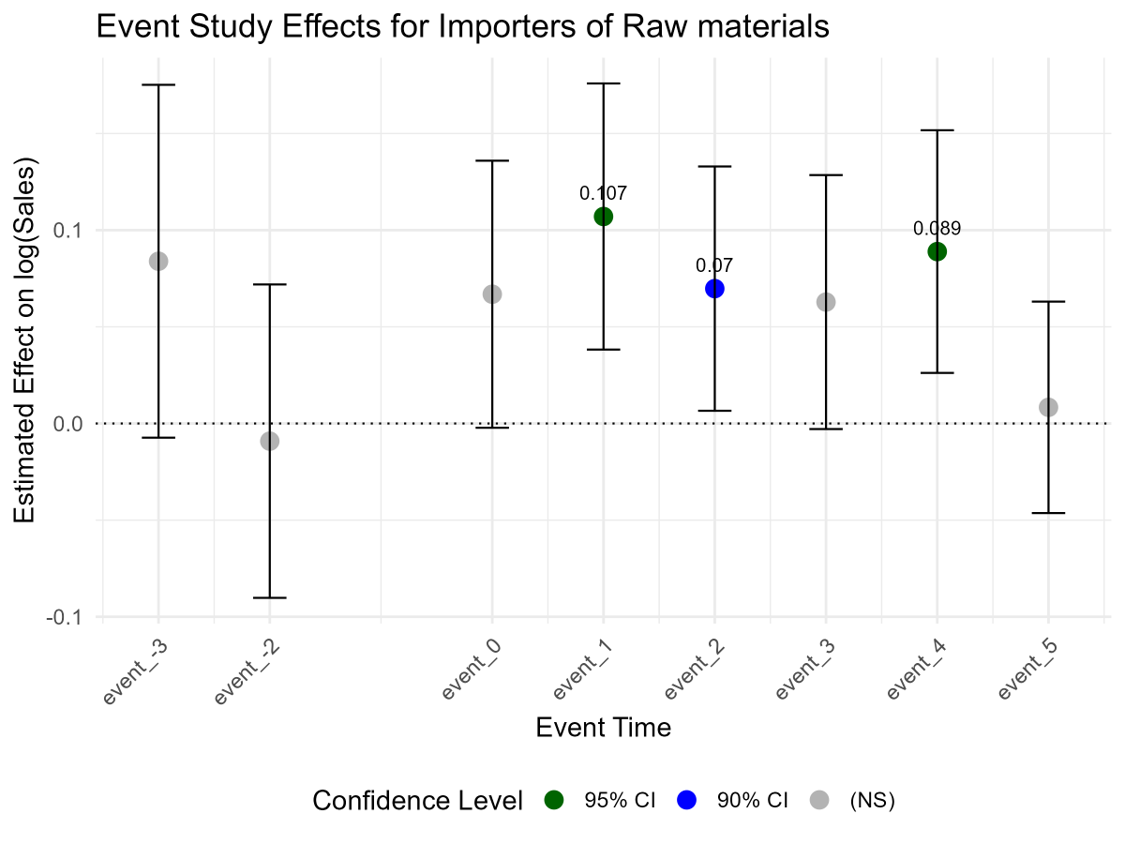
\includegraphics[width=\linewidth]{Results RawM.png}
\end{minipage}
\hfill
\begin{minipage}{0.49\textwidth}
    \centering
    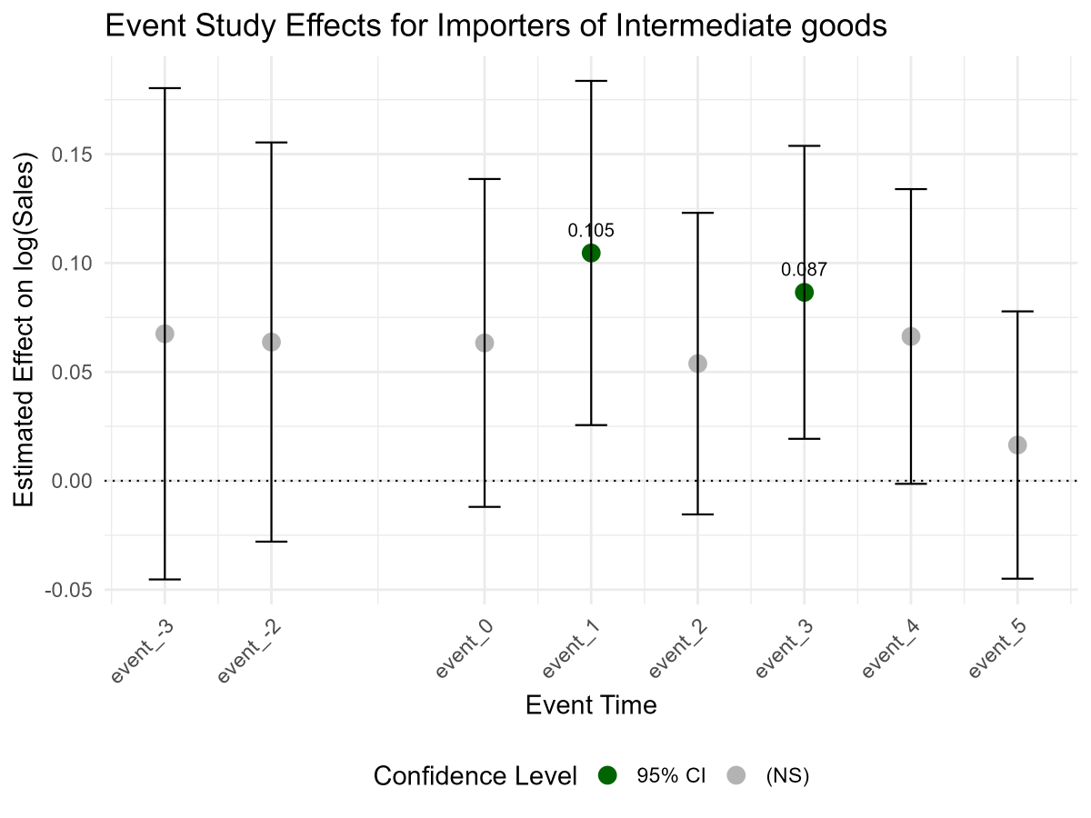
\includegraphics[width=\linewidth]{Results IntermIn.png}
\end{minipage}
\begin{itemize}
    \item Imports drive recovery
    \item Only specific imports matter (Raw materials, intermediate inputs)
    \item Sourcing from abroad mitigates damage (Increase of Sales by approx. 6\% to 10\%).
\end{itemize}
\end{frame}

\begin{frame}{Robustness -- Placebo tests}
\begin{itemize}
    \item \textbf{Alternative Outcomes} (wages, productivity, raw material expenses) consistent with the main findings
    \item \textbf{Placebo tests} \citep{Hagemann2019}: treatment year \& location randomized
\end{itemize}
\centering
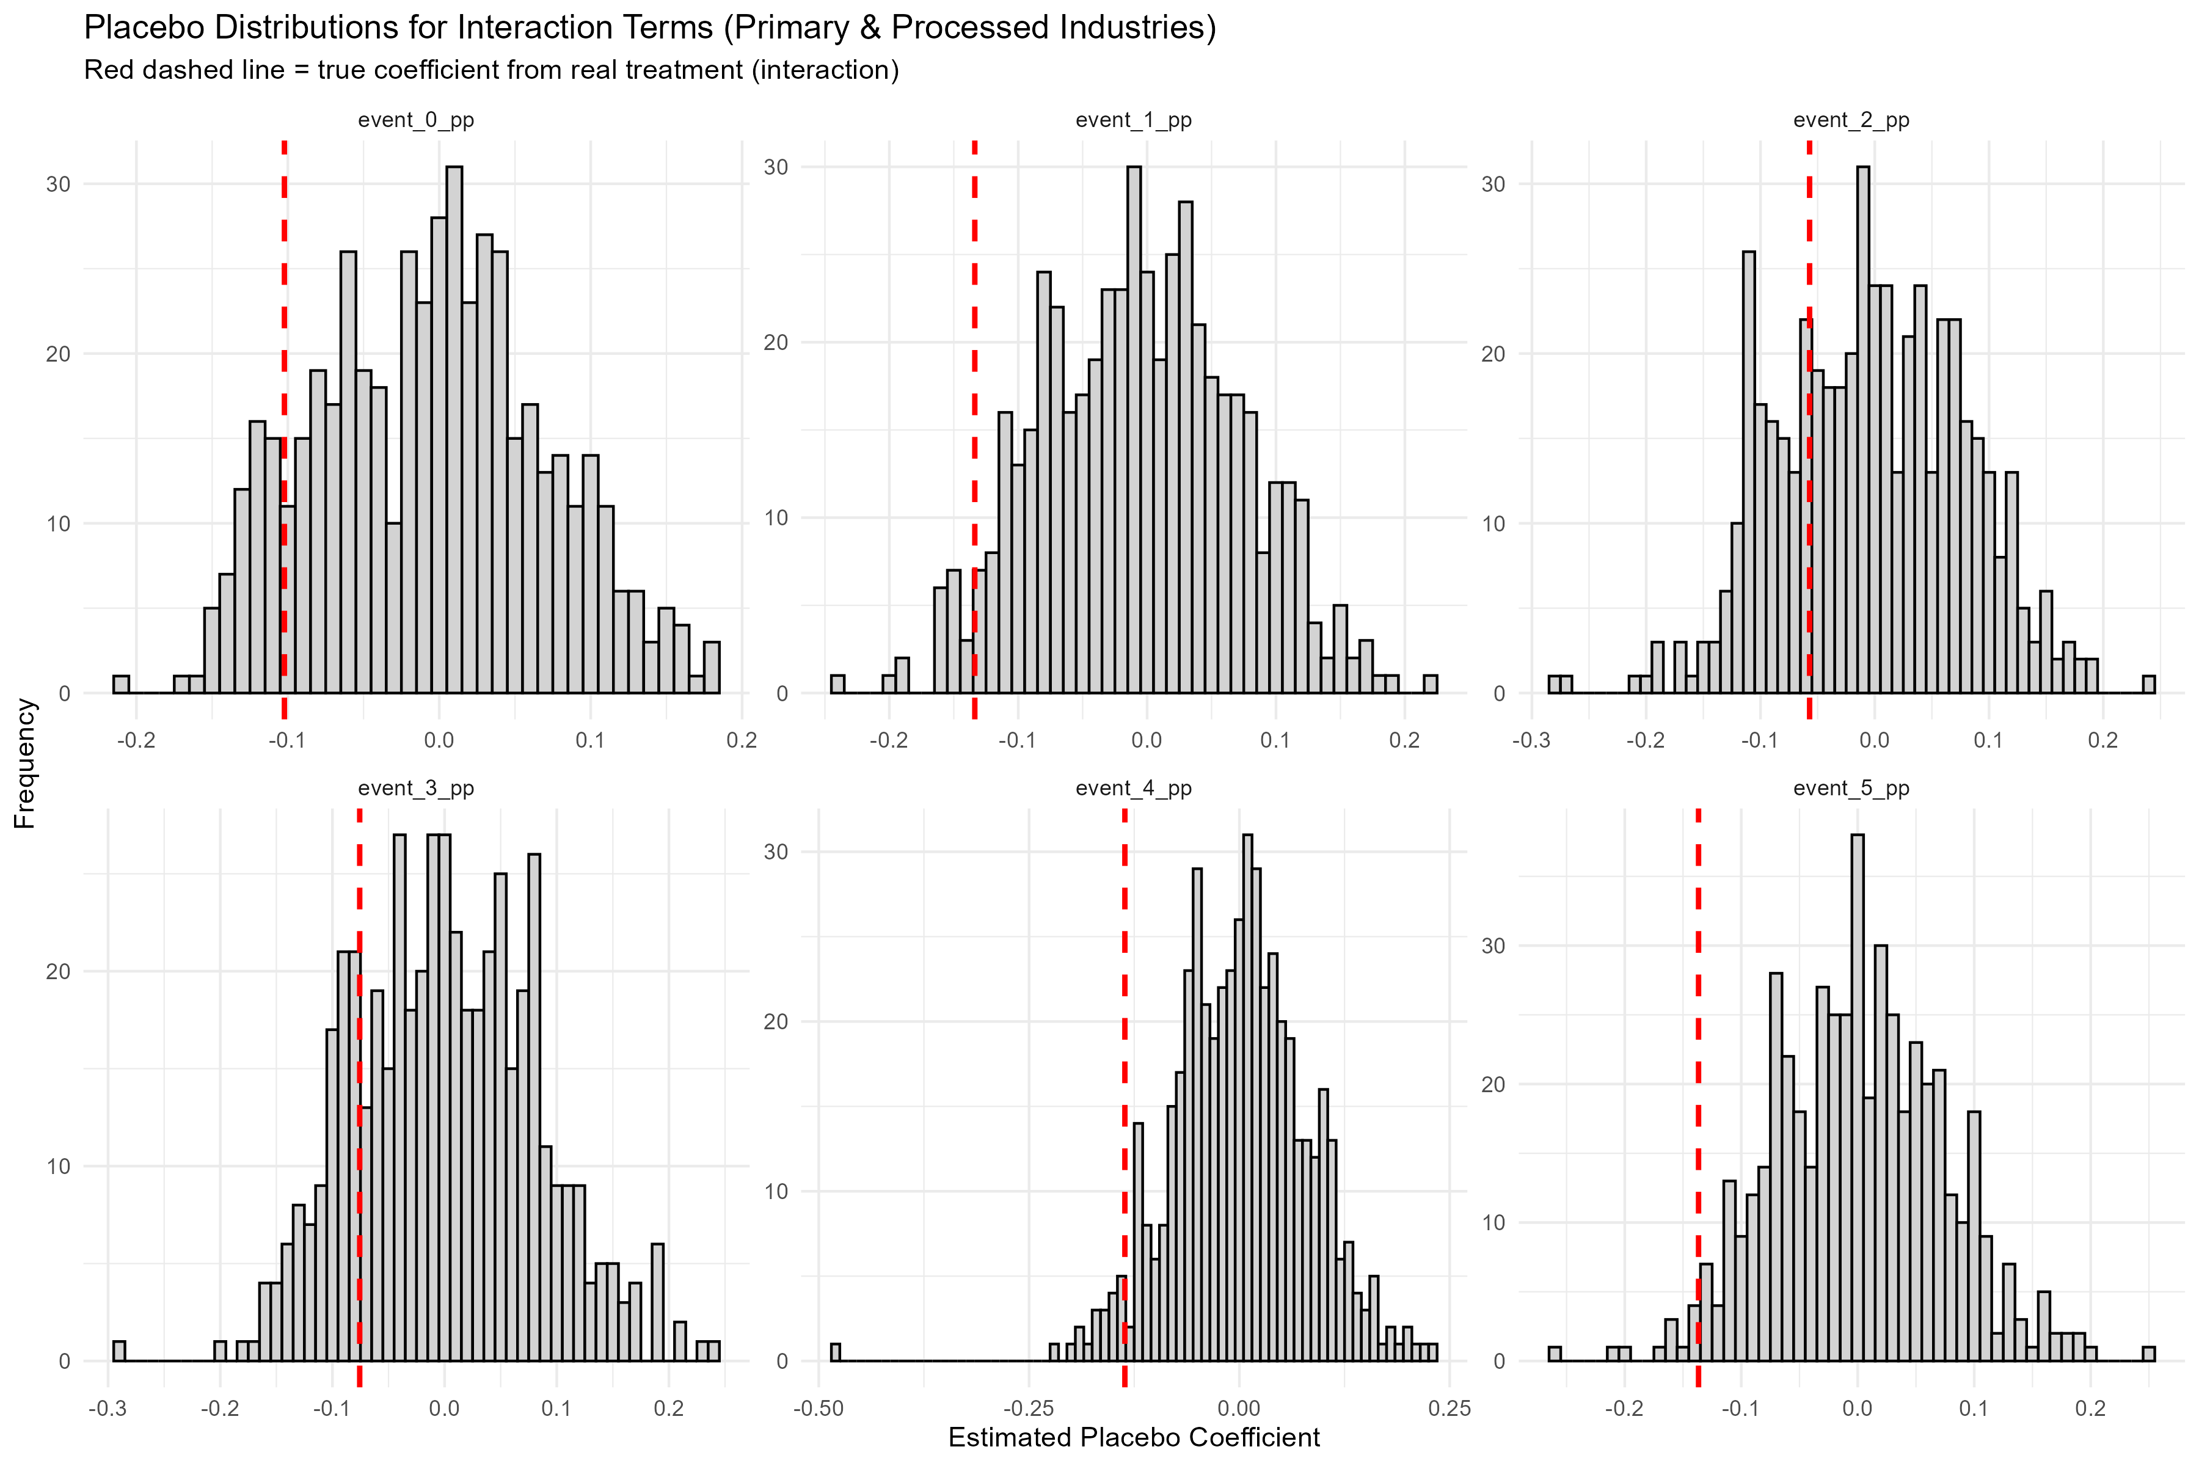
\includegraphics[height=5 cm]{Placebo distrib.png}
\end{frame}

\begin{frame}{Conclusion}
\begin{itemize}
\item \textbf{Discussions}
\begin{itemize}
    \item Data limitations (smaller firms + yearly period)
    \item Financial constraints
\end{itemize}
\item \textbf{To remember}
\begin{itemize}
    \item Natural disasters reduce firm performance, especially in upstream industries
    \item Imports can serve as a key adaptation mechanism
    \item Policy relevance: supporting trade and global input sourcing
\end{itemize}
\end{itemize}
\end{frame}

\begin{frame}
    \centering
    \Large Thank you!\\
    Feel free to ask any questions
\end{frame}

\begin{frame}{Appendices}
\vspace{-1cm}
\textbf{Composition of the Broader Sectors}
\begin{columns}

  \begin{column}{0.48\textwidth}
    
    \begin{itemize}
      \item \textbf{Primary \& Processed Products:} Food products, Wood products, Paper products, Books
      \item \textbf{Light Manufacturing:} Textiles, Leather products, Miscellaneous manufactured articles
      \item \textbf{Others:} Fall back category
    \end{itemize}
  \end{column}

  \begin{column}{0.48\textwidth}
    
    \begin{itemize}
      \item \textbf{Machinery \& Capital goods:} Machinery \& Machine tools, Transport equipment \& Parts
      \item \textbf{Chemicals \& Minerals:} Chemicals products, Non-Metallic Mineral products, Basic metals alloys \& metal products
      
    \end{itemize}
  \end{column}

\end{columns}
\end{frame}

\begin{frame}{Appendices}
\centering
    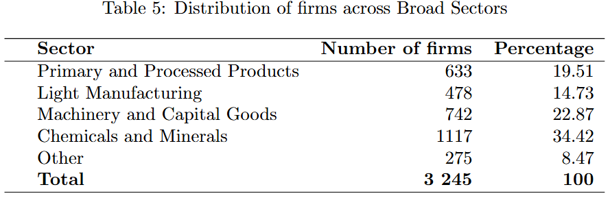
\includegraphics[height = 3.5 cm]{Firms distribution sectors.png}
    \vspace{0.3cm}
    \textbf{Main Industries}
    \begin{itemize}
    \item Machinery Tools (16\%)
    \item Chemical Products (15.7\%)
    \item Metal Products (14.8\%)
    \item Food Products (14.6\%)
    \item Textiles (13.5\%)
    \end{itemize}
\end{frame}

\begin{frame}{Appendices}
\centering
    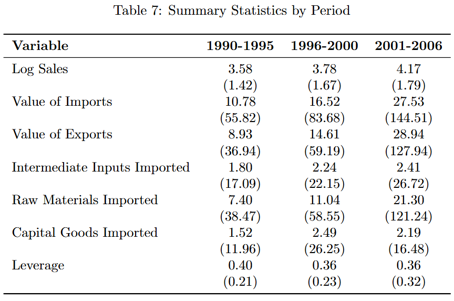
\includegraphics[height = 5 cm]{Summary stat time.png}
    \begin{itemize}
    \item Showing the growth trend of firms (context of trade liberalization and growth in the 1990s in India)
    \end{itemize}
\end{frame}

\begin{frame}{Appendices}
\centering
\begin{minipage}{0.49\textwidth}
    \centering
    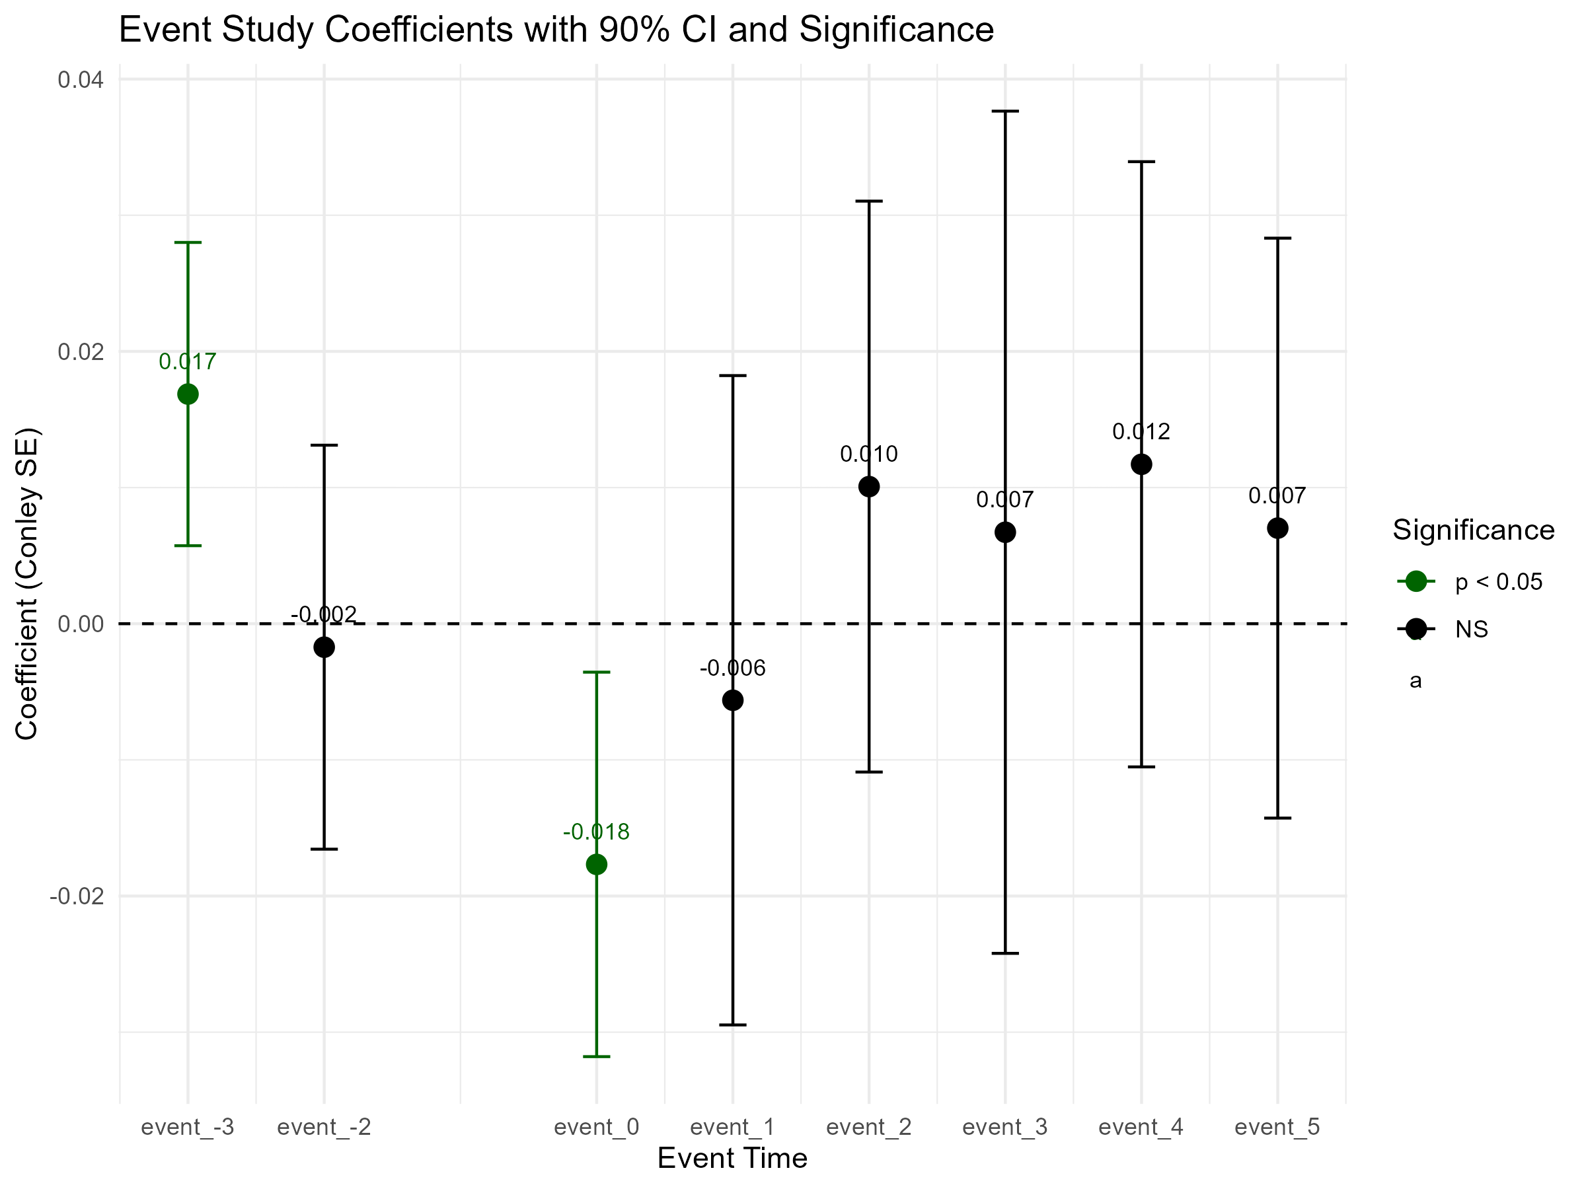
\includegraphics[width=\linewidth]{Results Pre Matching.png}
\end{minipage}
\hfill
\begin{minipage}{0.49\textwidth}
    \centering
    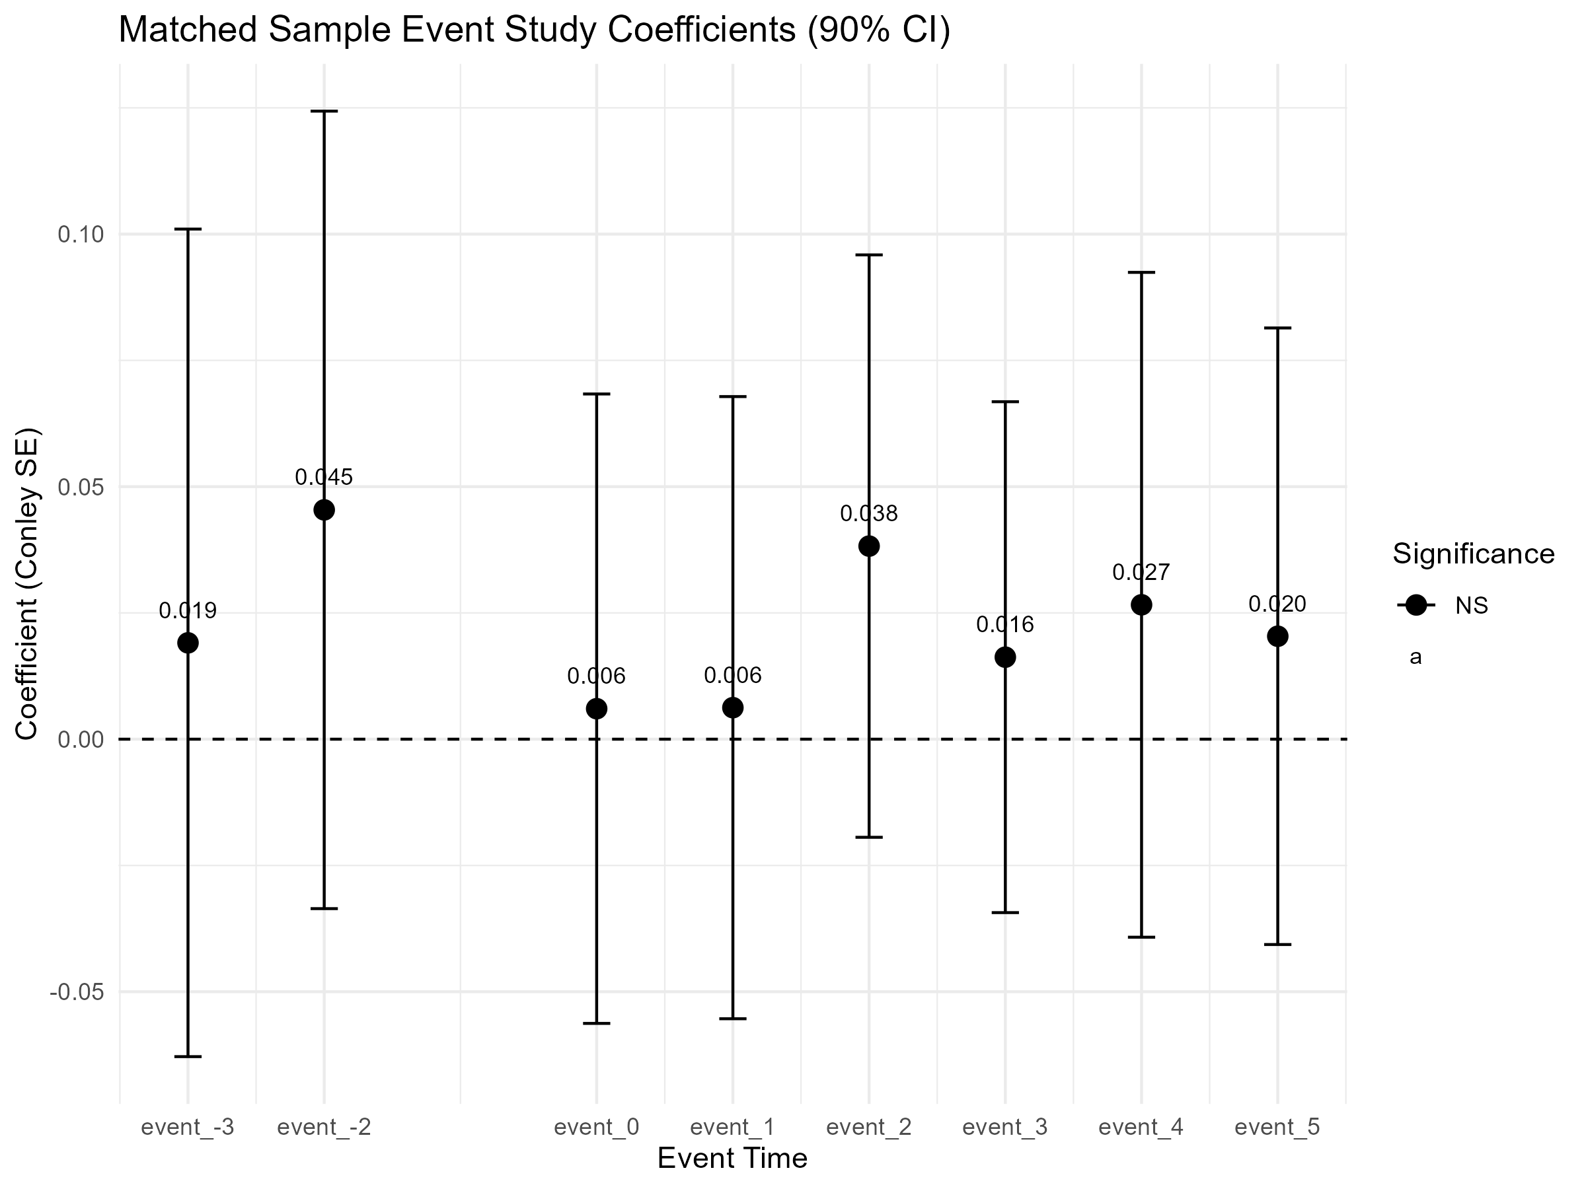
\includegraphics[width=\linewidth]{Results Post Matching.png}
\end{minipage}
\begin{itemize}
    \item Matching to remove pre-trends
    \item PSM based on a probit model
    \begin{itemize}
        \item Restrictive setup (method "nearest")
        \item Dropping Observations from 26k to 8.8k
    \end{itemize}
\end{itemize}
\end{frame}

\begin{frame}{Appendices}
    \centering
    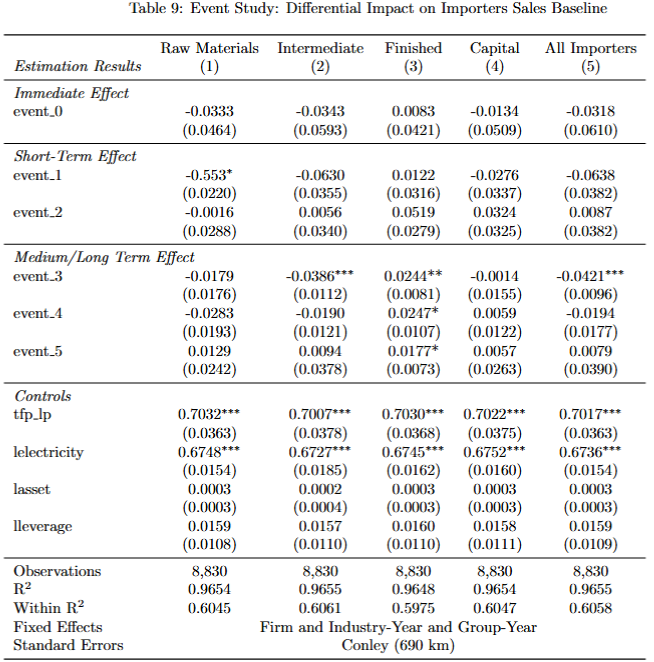
\includegraphics[height = 7 cm]{Baselines Importers.png}
    \begin{itemize}
        \item Baseline results for Importers
        \item To compare with non affected importers
    \end{itemize}
\end{frame}

\begin{frame}{Appendices}
    \centering
    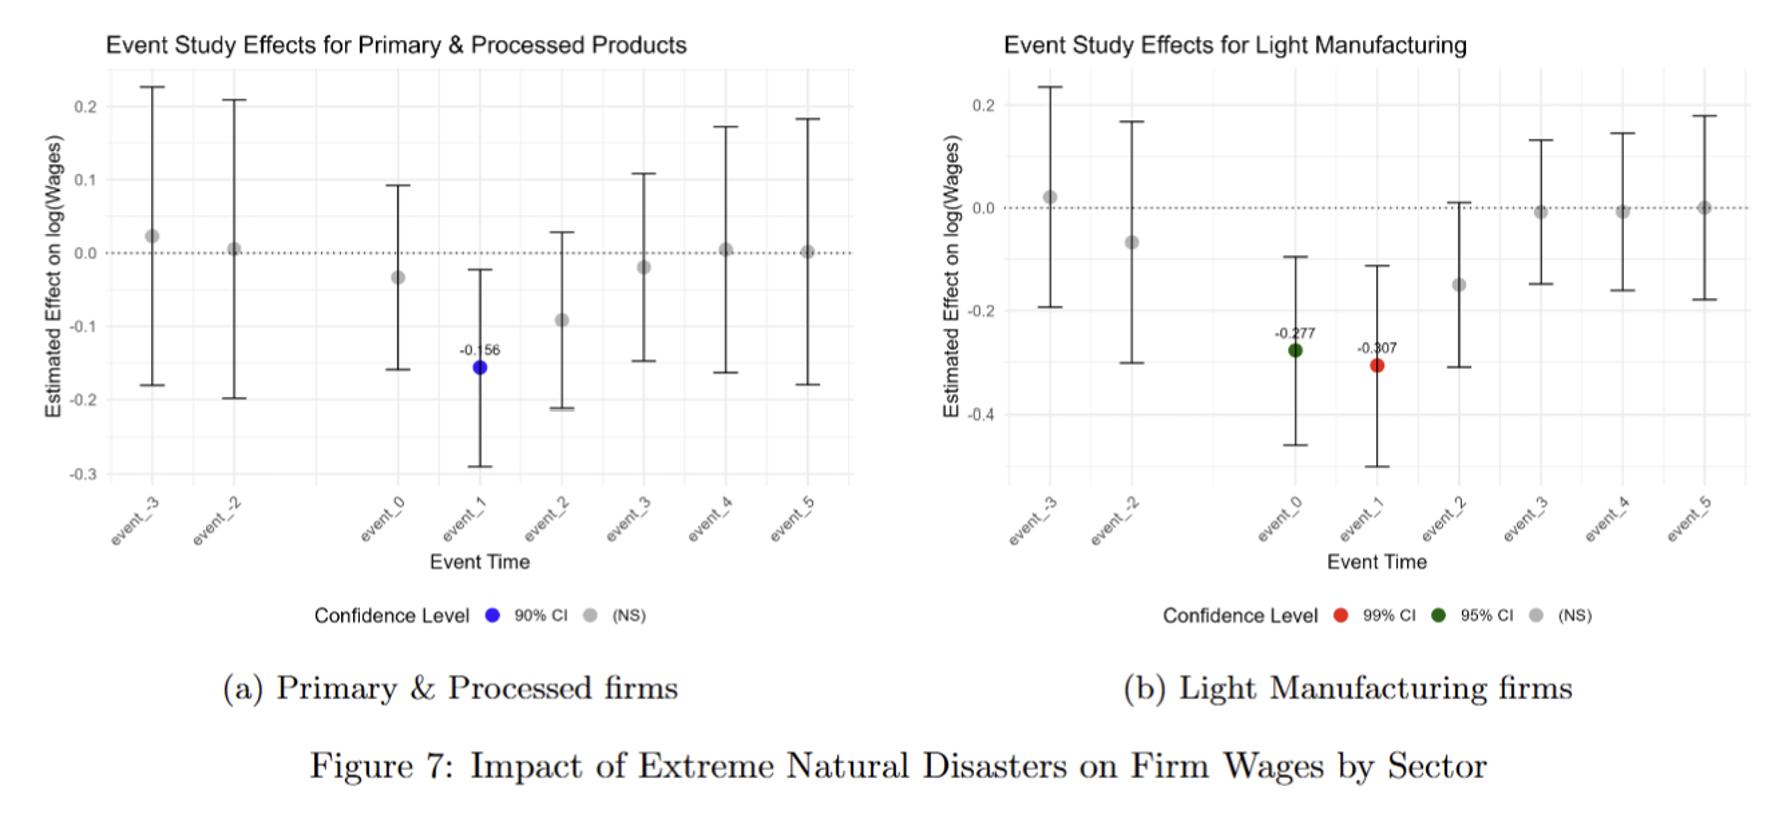
\includegraphics[height = 5.5 cm]{Results on Wages.png}
    \begin{itemize}
        \item Impact on wages
        \item Drop in the very short term
    \end{itemize}
\end{frame}

\begin{frame}{Appendices}
\vspace{-1.5cm}
\centering
\begin{minipage}{0.55\textwidth}
    \centering
    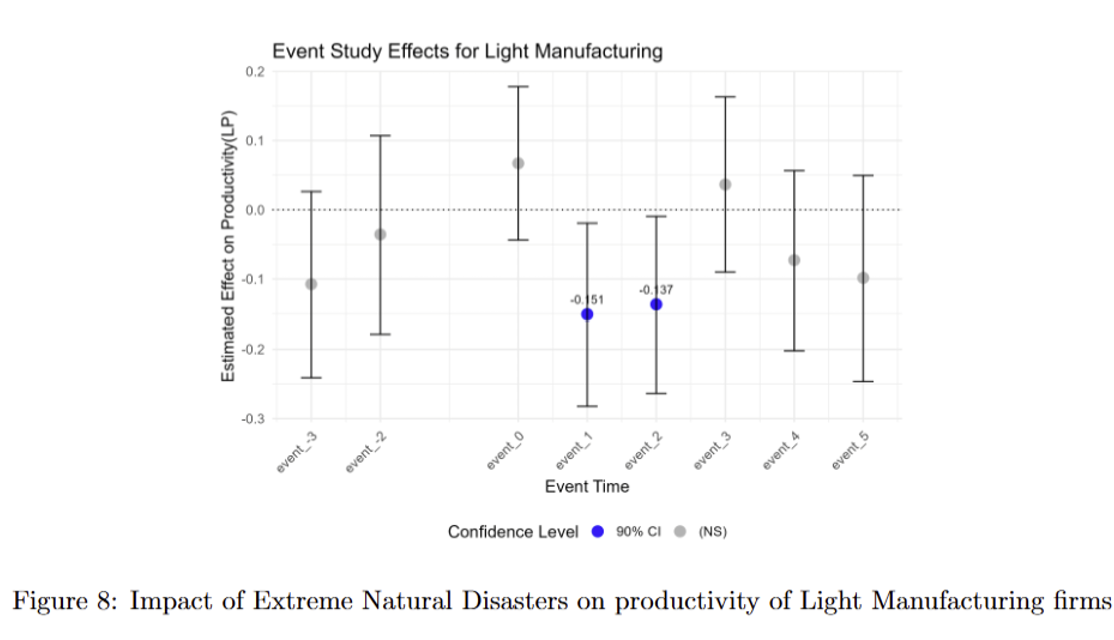
\includegraphics[width=\linewidth]{Results productivity.png}
\end{minipage}
\hfill
\begin{minipage}{0.60\textwidth}
    \centering
    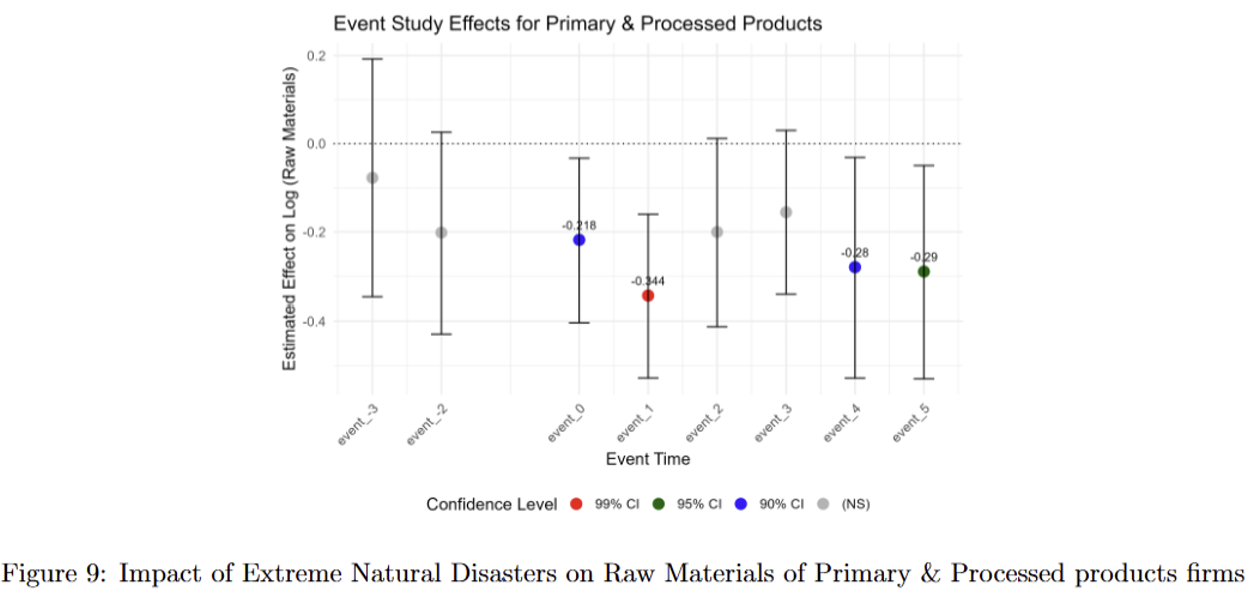
\includegraphics[width=\linewidth]{Results RawM exp.png}
\end{minipage}
\begin{itemize}
\scriptsize
    \item Impact on Productivity \& Raw Material expenses
    \item Upstream industries are the most affected 
\end{itemize}
\end{frame}


\bibliographystyle{apalike}
\bibliography{reference}


\end{document}
